\chapter{Implementation}
\label{chap:implementation}
\todo{Talk about how the deformation is done without mentioning springs first. I.e. you apply force to it.}
\todo{Also mention the importance of damping.}
\todo{Discuss semi-implicit euler integration scheme. Show math and implementation, discuss advantages and disadvantages with it.}

\section{Semi-Implicit Euler Integration}

\section{Spring Mesh Damping}
The spring mesh damping model is usually presented in a quite intuitive manner. 
Each vertex within a mesh is considered a point with its own mass. 
Between the vertices are springs which try to hold the whole mesh together.
When no forces are applied to the vertices within the model, the length of the springs are in their desired \rephrase{"resting" state.}
When a forces are applied to the vertices and they start moving, the springs holding the vertices together will become stretched
and will try to get back to their resting state.

\todo{Add image}

\section{Implicit Springs - Ball Deformation}
\todo{Add video}
\todo{Add how force is applied, showing the picture from the tutorial}
Jasper Flick\cite{catlike_mesh_deformation} shows an implementation \rephrase{without explicit springs}, following a semi-implicit euler integration scheme. 
In this implementation we keep a copy of the initial vertex positions, as well as a collection of the modified vertices.
Additionally, we keep a collection of the velocity of each vertex, which we update each time force is added to a vertex.
The springs come into play when updating the positions of all the vertices based on their velocities.
Each spring within this system is the vector between the initial positions of the vertices in the mesh and their current positions, as seen in figure \ref{fig:catlike_mesh_deformation_springs}.
Upon update of the vertices the force of a spring is applied to the velocity of a vertex in the direction of the spring, moving the vertex back towards its initial position (see listing~\ref{code:catlike_mesh_deformation_update}).

\begin{figure}
%\centering
    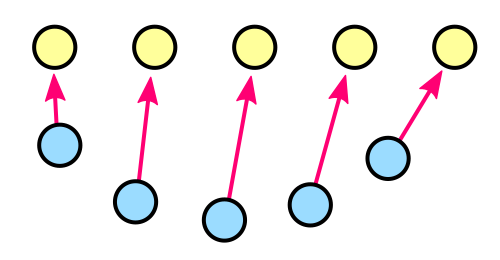
\includegraphics[width=\textwidth]{report/figures/catlike_mesh_deformation_springs.png}
    \caption{Modified vertices(yellow) are pulled towards their original position(blue) by the springs (pink)\cite{catlike_mesh_deformation}}
    \label{fig:catlike_mesh_deformation_springs}
\end{figure}

\begin{figure}
\begin{lstlisting}[label={code:catlike_mesh_deformation_update},language=csharp,caption={Catlike coding mesh deformation vertex update}]
private void UpdateVertex(int i)
{
    Vector3 velocity = mVertexVelocities[i];
    Vector3 spring = mDisplacedVertices[i] - mOriginalVertices[i];
    spring *= UniformScale; 
    velocity -= spring * SpringForce * Time.deltaTime;
    velocity *= 1f - Damping * Time.deltaTime;
    mVertexVelocities[i] = velocity;
    mDisplacedVertices[i] += velocity * (Time.deltaTime / UniformScale);
}
\end{lstlisting}
\end{figure}

\subsection{Usage}
As seen from the video, although simple, the implementation provides quite a lot of flexibility, toying with the different variables 
can lead to some interesting visual effects. 
For example, applying negative force to the sphere can be used to create a visual effect similar to that of a star being swallowed by a black hole.
Applying outward force from the inside of the model can create a relatively convincing effect of something moving around inside the object.
Giving the sphere a high SpringForce will lead to it being harder to deform, and more bouncy when trying to return to its original shape.

\subsection{Limitations}
As previously mentioned the implementation is quite simple, but has some limitations. 
As mentioned by Flick\cite{catlike_mesh_deformation} this implementation is not a physics simulation, while the mesh is deformed
the colliders and physical representation of the object stays the same.
Additionally, none of the vertices are connected to each other through springs, and therefore move completely independent from each other. 
This means that if we were to for instance pin two of the vertices to their initial position, and then apply force to the mesh
none of the other vertices would respect that two of them was locked in place, leading to less than satisfying results.

\section{Verlet Integration}
\todo{Discuss Verlet Integration}

\section{Explicit Springs - Cloth Simulation}
Cloth simulation is a place where the springs are more apparent than the previous implementation.
The implementation seen in Figure \ref{fig:my_cloth_implementation_springs} shows all the springs needed to create a believable cloth simulation.
The implementation is based on the implementation shown by Jesper Mosegaard\cite{mosegaards_clothing_simulation}.
Unlike the previous implementation, the springs here are explicit and ensure that vertices are not handled in isolation but rather are affected by the other vertices in the system.
This gives greater control in that it allows you to apply force to a specific vertex and the whole system responds, rather than having to apply the force to all the vertices.
\think{Need to start to segue into the spring types}

\todo{Find the gamasutra article that discussed this}


\begin{figure}
%\centering
    \caption{\todo{Insert figure}}
    \label{fig:my_cloth_implementation_springs}
\end{figure}


\subsection{Spring Types}
\subsubsection{Structural Springs}

\subsubsection{Shear Springs}

\subsubsection{Bending Springs}



\todo{We should be able to cut the cloth mesh without any problems right? as long as we "cut" along the triangles, so that no triangle reference a part that has been cut off}



\todo{The technology ahead, ask if this could be used with tesselation and be done on the GPU?}
